\documentclass[xetex,mathserif,serif]{beamer}
\usepackage{polyglossia}
\setdefaultlanguage[babelshorthands=true]{russian}
\usepackage{minted}
\usepackage{tabu}

\useoutertheme{infolines}

\usepackage{fontspec}
\setmainfont{FreeSans}
\newfontfamily{\russianfonttt}{FreeSans}

\setbeamertemplate{blocks}[rounded][shadow=false]

\setbeamercolor*{block title alerted}{fg=red!50!black,bg=red!20}
\setbeamercolor*{block body alerted}{fg=black,bg=red!10}

\tabulinesep=1.2mm

\title{Многопоточное программирование}
\subtitle{Часть 1: высокоуровневая многопоточность}
\author[Юрий Литвинов]{Юрий Литвинов\\\small{\textcolor{gray}{yurii.litvinov@gmail.com}}}
\date{8}

\newcommand{\todo}[1] {
	\begin{center}\textcolor{red}{TODO: #1}\end{center}
}

\newcommand{\DownArrow} {
	\hspace{2cm}\begin{LARGE}$\downarrow$\end{LARGE}
}

\begin{document}

	\frame{\titlepage}

	\section{Введение}

	\begin{frame}
		\frametitle{Многопоточное программирование вообще}
		\begin{itemize}
			\item Плюсы
			\begin{itemize}
				\item Не вешать пользовательский интерфейс
				\item Равномерно распределять вычислительно сложные задачи по ядрам
				\item Выполнять одновременно несколько блокирующих операций ввода-вывода
			\end{itemize}
			\item Минусы
			\begin{itemize}
				\item Тысяча способов прострелить себе ногу
				\item Не всегда многопоточная программа работает быстрее однопоточной
			\end{itemize}
		\end{itemize}
	\end{frame}

	\begin{frame}
		\frametitle{Race condition}
		\begin{center}
			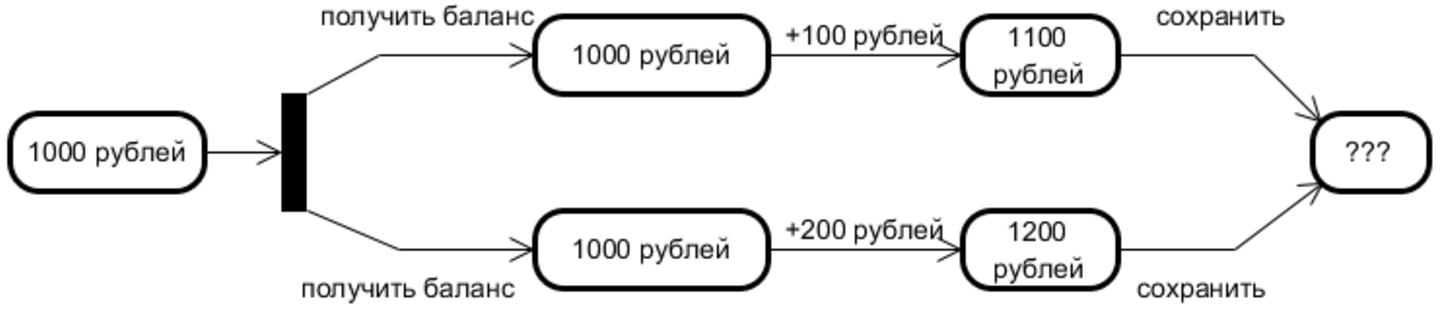
\includegraphics[width=0.9\textwidth]{raceCondition.png}
		\end{center}
	\end{frame}

	\begin{frame}
		\frametitle{Deadlock}
		\begin{center}
			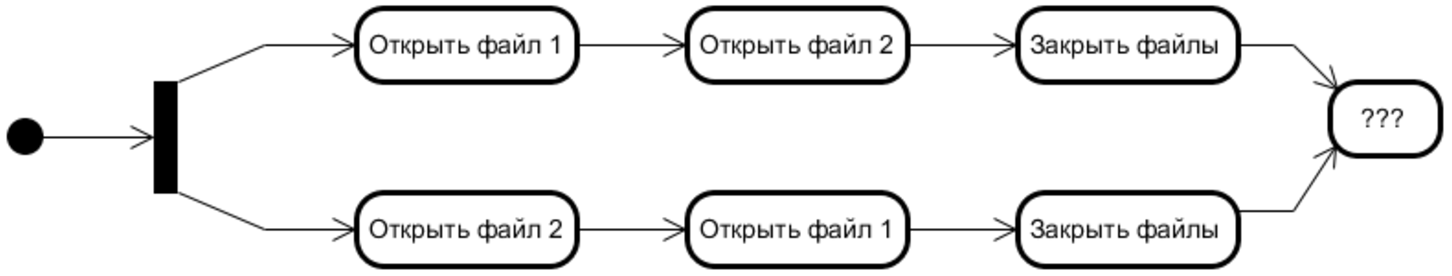
\includegraphics[width=0.9\textwidth]{deadlock.png}
		\end{center}
	\end{frame}

	\section{Потоки в Windows}

	\begin{frame}
		\frametitle{Поток в Windows}
		\begin{itemize}
			\item Thread Kernel Object (~1240 байт)
			\item Thread environment block (TEB) (4 Кб)
			\item User-mode stack (1 Мб)
			\item Kernel-mode stack (24 Кб)			
		\end{itemize}

		Ещё для каждой dll-ки, загруженной для процесса при старте или остановке потока вызывается DllMain с параметрами DLL\_THREAD\_ATTACH и DLL\_THREAD\_DETACH

		\vspace{3mm}
		Квант времени --- ~20-30 мс, после чего происходит \textit{переключение контекстов}
	\end{frame}

	\begin{frame}
		\frametitle{Как делать не надо}
		\begin{center}
			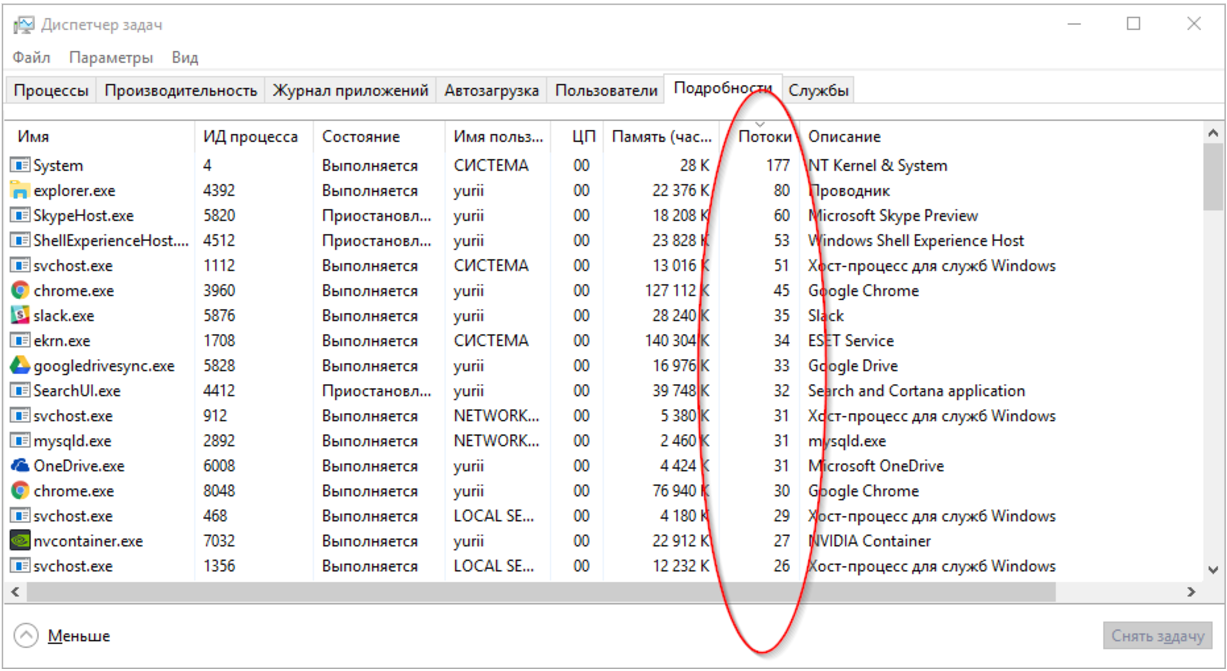
\includegraphics[width=0.9\textwidth]{threadsEverywhere.png}
		\end{center}
	\end{frame}

	\begin{frame}[fragile]
		\frametitle{System.Threading.Thread}
		\begin{minted}{csharp}
Thread dedicatedThread = new Thread(ComputeBoundOp);
dedicatedThread.Start(5);
Thread.Sleep(10000);  // Симуляция 10 секунд какой-то работы
dedicatedThread.Join();  // Ждём второй поток
...

private static void ComputeBoundOp(Object state) {
    Console.WriteLine($"In ComputeBoundOp: state={state}");
    Thread.Sleep(1000);  // Симуляция секунды каких-то вычислений
}
		\end{minted}
	\end{frame}

	\begin{frame}
		\frametitle{Планировщик}
		\begin{itemize}
			\item Раз в квант времени (или чаще) выбирает поток для исполнения
			\begin{itemize}
				\item Рассматриваются только потоки, не ждущие чего-либо
			\end{itemize}
			\item НЕ реальное время
			\begin{itemize}
				\item Нельзя делать предположения, когда потоку дадут поработать
			\end{itemize}
			\item Из рассматриваемых потоков выбираются только те, у кого наибольший приоритет
			\begin{itemize}
				\item Приоритеты потоков от 0 до 31, обычно 8
			\end{itemize}
			\item Есть ещё приоритеты процессов: Idle, Below, Normal, Normal, Above Normal, High и Realtime
			\item Относительные приоритеты потоков: Idle, Lowest, Below Normal, Normal, Above Normal, Highest и Time-Critical
			\begin{itemize}
				\item Истинный приоритет получается из относительного приоритета и приоритета процесса
			\end{itemize}
		\end{itemize}
	\end{frame}

	\begin{frame}[fragile]
		\frametitle{Foreground- и Background-потоки}
		\begin{itemize}
			\item Когда все Foreground-потоки завершили работу, рантайм останавливает все Background-потоки и заканчивает работу приложения
			\item Thread по умолчанию создаётся как Foreground
			\begin{itemize}
				\item Способ прострелить себе ногу №1: создать foreground-поток и забыть о нём, приложение будет висеть в списке задач и не завершится
			\end{itemize}
		\end{itemize}
		\vspace{5mm}
		Способ прострелить себе ногу №2: создать background-поток и не дать ему доработать:
		\begin{minted}{csharp}
Thread t = new Thread(Worker);
t.IsBackground = true;
t.Start();
Console.WriteLine("Returning from Main");
		\end{minted}
	\end{frame}

	\section{Пул потоков}

	\begin{frame}
		\frametitle{Пул потоков}
		\begin{itemize}
			\item Содержит набор заранее созданных потоков, которые могут исполнять задачи
			\item Управляется рантаймом
			\begin{itemize}
				\item Новые потоки создаются при необходимости
				\item Потоки автоматически удаляются, если они долго не используются и потоков больше, чем надо
				\item ``Сколько надо'' рантайм определяет по количеству доступных ядер процессора
			\end{itemize}
			\item Используется в .NET практически повсеместно
			\begin{itemize}
				\item Идеологически многопоточное приложение оперирует не потоками, а задачами и асинхронными операциями
			\end{itemize}
			\item Все потоки из пула --- Background
		\end{itemize}
	\end{frame}

	\begin{frame}[fragile]
		\frametitle{Пример}
		\begin{minted}{csharp}
public static void Main() {
    Console.WriteLine("Main thread: queuing an asynchronous operation");
    ThreadPool.QueueUserWorkItem(ComputeBoundOp, 5);
    Console.WriteLine("Main thread: Doing other work here...");
    Thread.Sleep(10000);  // Симуляция работы в главном потоке
    Console.WriteLine("Hit <Enter> to end this program...");
    Console.ReadLine();
}

private static void ComputeBoundOp(Object state) {
    Console.WriteLine("In ComputeBoundOp: state={0}", state);
    Thread.Sleep(1000);  // Симуляция работы в потоке из пула
}
		\end{minted}
	\end{frame}

	\begin{frame}[fragile]
		\frametitle{Контекст исполнения}
		\begin{footnotesize}
			Ассоциированная с потоком структура данных, где хранятся разные свойства потока (например, свойства безопасности):
			\begin{minted}{csharp}
public static void Main() {
    CallContext.LogicalSetData("Name", "Jeffrey");
    ThreadPool.QueueUserWorkItem(
        state => Console.WriteLine("Name={0}", CallContext.LogicalGetData("Name")));
    ExecutionContext.SuppressFlow();
    ThreadPool.QueueUserWorkItem(
        state => Console.WriteLine("Name={0}", CallContext.LogicalGetData("Name")));
    ExecutionContext.RestoreFlow();
    ...
    Console.ReadLine();
}
			\end{minted}
		\end{footnotesize}
	\end{frame}

	\begin{frame}
		\frametitle{Отмена операций}
		\begin{itemize}
			\item CancellationToken --- отдаётся потоку, он должен сам проверять состояние токена и прерваться, если запрошена отмена
			\begin{itemize}
				\item Может прерваться не мгновенно, проверка возможна только время от времени
			\end{itemize}
			\item CancellationTokenSource --- умеет производить CancellationToken-ы, может выставлять флаг отмены для всех созданных CancellationToken-ов, остаётся в основном потоке
		\end{itemize}
	\end{frame}

	\begin{frame}[fragile]
		\frametitle{Пример}
		\begin{small}
			\begin{minted}{csharp}
public static void Main() {
    CancellationTokenSource cts = new CancellationTokenSource();
    ThreadPool.QueueUserWorkItem(o => Count(cts.Token, 1000));
    Console.ReadLine();
    cts.Cancel();
    Console.ReadLine();
}

private static void Count(CancellationToken token, Int32 countTo) {
    for (Int32 count = 0; count < countTo; count++) {
        if (token.IsCancellationRequested) {
            break;
        }
       Thread.Sleep(200); 
    }
}
			\end{minted}
		\end{small}
	\end{frame}

	\begin{frame}[fragile]
		\frametitle{Полезные вещи CancellationToken}
		\begin{itemize}
			\item \mintinline{csharp}|CancellationToken.None|
			\item \mintinline{csharp}|CancellationToken.Register|:
				\begin{minted}{csharp}
var cts = new CancellationTokenSource();
cts.Token.Register(() => Console.WriteLine("Canceled 1"));
cts.Token.Register(() => Console.WriteLine("Canceled 2"));
				\end{minted}
				\begin{itemize}
					\item Возвращает \mintinline{csharp}|CancellationTokenRegistration|, реализующий \mintinline{csharp}|IDisposable|
				\end{itemize}
			\item \mintinline{csharp}|CancellationTokenSource.CreateLinkedTokenSource|
			\item \mintinline{csharp}|CancellationTokenSource.CancelAfter|
		\end{itemize}
	\end{frame}

	\section{Task}

	\begin{frame}[fragile]
		\frametitle{Task}
		\begin{itemize}
			\item Абстракция задачи, которая может быть выполнена в отдельном потоке
			\item Эквивалентные строки кода:
				\begin{minted}{csharp}
ThreadPool.QueueUserWorkItem(ComputeBoundOp, 5);
new Task(ComputeBoundOp, 5).Start();
Task.Run(() => ComputeBoundOp(5));
				\end{minted}
			\item Позволяет ждать окончание задачи и получать результат
			\item Тоже важен для реализации некоторых вещей в C\#, но часто используется и независимо
		\end{itemize}
	\end{frame}

	\begin{frame}[fragile]
		\frametitle{Пример}
		\begin{footnotesize}
			\begin{minted}{csharp}
private static Int32 Sum(Int32 n) {
    Int32 sum = 0;
    for (; n > 0; n--)
        checked { sum += n; } 
    return sum;
}
...
Task<Int32> t = new Task<Int32>(n => Sum((Int32)n), 1000000000);
t.Start();
t.Wait();  // t.Result сам делает Wait(), так что тут это только для иллюстрации
Console.WriteLine("The Sum is: " + t.Result);
			\end{minted}
		\end{footnotesize}
	\end{frame}

	\begin{frame}[fragile]
		\frametitle{Отмена Task-а}
		\begin{minted}{csharp}
private static Int32 Sum(CancellationToken ct, Int32 n) {
    Int32 sum = 0;
    for (; n > 0; n--) {
        ct.ThrowIfCancellationRequested();
        checked { sum += n; } 
    }
    return sum;
}
		\end{minted}
		\vspace{3mm}
		Кидает \mintinline{csharp}|OperationCanceledException| в основной поток при обращении к результату (на самом деле, \mintinline{csharp}|AggregateException| с \mintinline{csharp}|OperationCanceledException|)
	\end{frame}

	\begin{frame}[fragile]
		\frametitle{Полезные вещи Task-а}
		\begin{scriptsize}
			\begin{itemize}
				\item \mintinline{csharp}|ContinueWith|:
					\begin{minted}{csharp}
Task<Int32> t = Task.Run(() => Sum(CancellationToken.None, 10000));
Task cwt = t.ContinueWith(task => Console.WriteLine("The sum is: " + task.Result));
					\end{minted}
				\item Родительские задачи:
					\begin{minted}{csharp}
Task<Int32[]> parent = new Task<Int32[]>(() => {
    var results = new Int32[3];
    new Task(() => results[0] = Sum(10000), TaskCreationOptions.AttachedToParent).Start();
    new Task(() => results[1] = Sum(20000), TaskCreationOptions.AttachedToParent).Start();
    new Task(() => results[2] = Sum(30000), TaskCreationOptions.AttachedToParent).Start();
    return results;
});
var cwt = parent.ContinueWith(
        parentTask => Array.ForEach(parentTask.Result, Console.WriteLine));
					\end{minted}
			\end{itemize}
		\end{scriptsize}
	\end{frame}

	\begin{frame}[fragile]
		\frametitle{TaskFactory}
		\begin{minted}{csharp}
var cts = new CancellationTokenSource();
var tf = new TaskFactory<Int32>(cts.Token,   
        TaskCreationOptions.AttachedToParent,
        TaskContinuationOptions.ExecuteSynchronously, 
        TaskScheduler.Default);

    var childTasks = new[] {
    tf.StartNew(() => Sum(cts.Token, 10000)),
    tf.StartNew(() => Sum(cts.Token, 20000)),
    tf.StartNew(() => Sum(cts.Token, Int32.MaxValue)) 
};
		\end{minted}
	\end{frame}

	\begin{frame}[fragile]
		\frametitle{TaskScheduler}
		\begin{itemize}
			\item Класс, позволяющий управлять тем, как Task-и обрабатываются пулом потоков (и пулом потоков ли вообще)
			\begin{itemize}
				\item По умолчанию таски ставятся в очередь в пуле потоков
			\end{itemize}
			\item Бывает полезно, например, чтобы задача могла модифицировать элементы GUI
			\begin{itemize}
				\item Это можно делать только из главного потока (который создал GUI)
			\end{itemize}
		\end{itemize}

		\begin{small}
			\begin{minted}{csharp}
Task<Int32> t = Task.Run(() => Sum(m_cts.Token, 20000), m_cts.Token);
t.ContinueWith(task => Text = "Result: " + task.Result,
        CancellationToken.None,
        TaskContinuationOptions.OnlyOnRanToCompletion,
        TaskScheduler.FromCurrentSynchronizationContext());
			\end{minted}
		\end{small}
	\end{frame}

	\begin{frame}[fragile]
		\frametitle{Более высокоуровневые вещи}
		\begin{minted}{csharp}
for (Int32 i = 0; i < 1000; i++) DoWork(i);
		\end{minted}
		\DownArrow
		\begin{minted}{csharp}
Parallel.For(0, 1000, i => DoWork(i));
		\end{minted}

		Есть ещё:
		\begin{itemize}
			\item \mintinline{csharp}|Parallel.ForEach(collection, item => DoWork(item));|
			\item 
				\begin{minted}{csharp}
Parallel.Invoke(
    () => Method1(),
    () => Method2(),
    () => Method3());
				\end{minted}
			\item \mintinline{csharp}|ParallelQuery<T>| и LINQ
		\end{itemize}
	\end{frame}

	\section{async/await}

	\begin{frame}
		\frametitle{async/await}
		\begin{columns}
			\begin{column}{0.5\textwidth}
				\begin{itemize}
					\item Task и пул потоков хороши для дорогих по времени операций
					\item Чаще поток ждёт окончания операции ввода-вывода
					\item Блокирующий ввод-вывод ``вешает'' поток, заставляя пул потоков создавать новые
				\end{itemize}
			\end{column}
			\begin{column}{0.5\textwidth}
				\begin{center}
					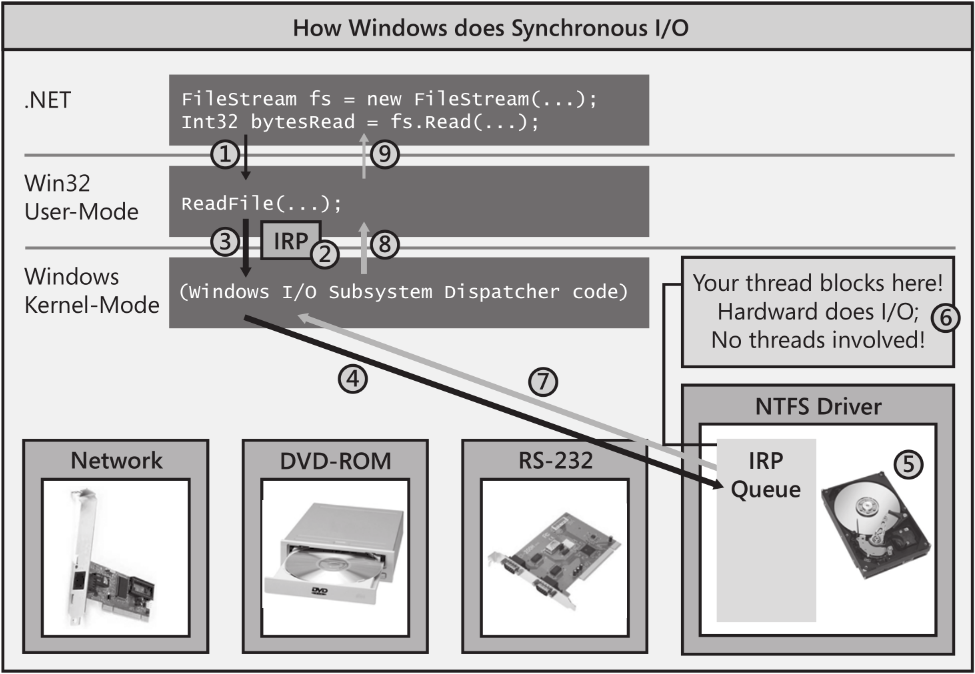
\includegraphics[width=0.9\textwidth]{windowsSynchronousIO.png}
					
					\begin{footnotesize}(Рисунок из Jeffrey Richter. CLR via C\#)\end{footnotesize}
				\end{center}
			\end{column}
		\end{columns}
	\end{frame}

	\begin{frame}
		\frametitle{async/await (2)}
		\begin{columns}
			\begin{column}{0.5\textwidth}
				\begin{itemize}
					\item Асинхронные операции ввода-вывода не блокируют поток, возвращая управление тут же
					\begin{itemize}
						\item Данные, естественно, не готовы
					\end{itemize}
					\item Старая модель в .NET --- \mintinline{csharp}|Begin...()| и \mintinline{csharp}|End...()|
					\begin{itemize}
						\item \mintinline{csharp}|Begin...()| инициирует операцию, принимая колбэк, где можно использовать \mintinline{csharp}|End...()|, чтобы забрать результат
					\end{itemize}
				\end{itemize}
			\end{column}
			\begin{column}{0.5\textwidth}
				\begin{center}
					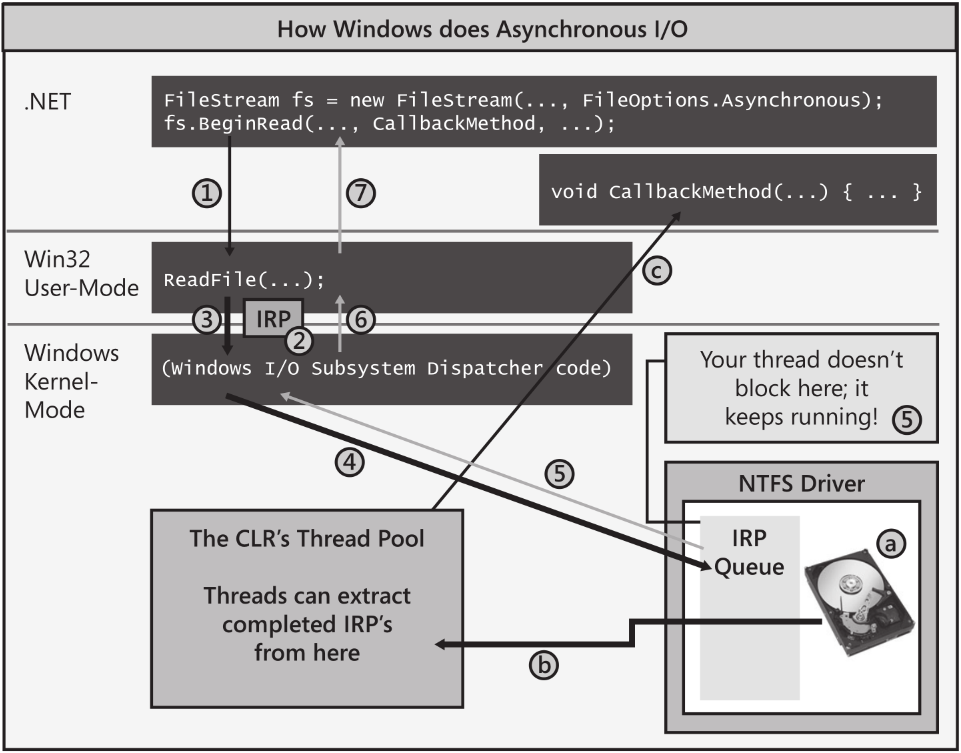
\includegraphics[width=0.9\textwidth]{windowsAsynchronousIO.png}

					\begin{footnotesize}(Рисунок из Jeffrey Richter. CLR via C\#)\end{footnotesize}
				\end{center}
			\end{column}
		\end{columns}
	\end{frame}

	\begin{frame}
		\frametitle{async/await (3)}
		\begin{columns}
			\begin{column}{0.5\textwidth}
				\begin{itemize}
					\item Новая модель: async/await
					\item Требуется поддержка компилятора
					\item Можно понимать как сопрограмму
					\item На самом деле, генерируется конечный автомат
					\begin{itemize}
						\item Запоминает, на каком await сейчас мы находимся
						\item Следит за исключениями
					\end{itemize}
				\end{itemize}
			\end{column}
			\begin{column}{0.5\textwidth}
				\begin{center}
					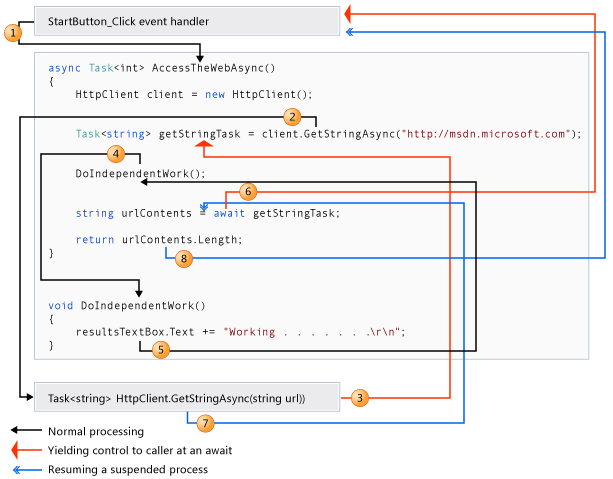
\includegraphics[width=0.9\textwidth]{asyncAwait.png}

					\begin{footnotesize}(Рисунок из \href{https://msdn.microsoft.com/library/hh191443(vs.110).aspx}{MSDN})\end{footnotesize}
				\end{center}
			\end{column}
		\end{columns}
	\end{frame}

	\begin{frame}[fragile]
		\frametitle{Пример}
		\begin{small}
			\begin{minted}{csharp}
internal sealed class Type1 { }
internal sealed class Type2 { }
private static async Task<Type1> Method1Async() { ... }
private static async Task<Type2> Method2Async() { ... }

private static async Task<String> MyMethodAsync(Int32 argument) {
    Int32 local = argument;
    try {
        Type1 result1 = await Method1Async();
        for (Int32 x = 0; x < 3; x++) {
            Type2 result2 = await Method2Async();
        }
    }
    catch (Exception) { Console.WriteLine("Catch"); }
    return "Done";
}
			\end{minted}
		\end{small}
	\end{frame}

	\begin{frame}
		\frametitle{Особенности}
		\begin{itemize}
			\item Может возвращать только \mintinline{csharp}|Task|, \mintinline{csharp}|Task<Result>| или \mintinline{csharp}|void|
			\begin{itemize}
				\item \mintinline{csharp}|void| используется для асинхронных обработчиков событий
			\end{itemize}
			\item Любой Task можно ждать await-ом, любой async можно не ждать
			\begin{itemize}
				\item Вызов Result у результата async-метода заставляет его исполниться синхронно
			\end{itemize}
			\item Работает только с .NET 4.5 и C\# 5
			\begin{itemize}
				\item Microsoft.BCL, если надо поддержать более старый рантайм
			\end{itemize}
		\end{itemize}
	\end{frame}

	\begin{frame}
		\frametitle{Async-методы в стандартной библиотеке}
		\begin{itemize}
			\item \mintinline{csharp}|System.IO.Stream| и потомки: \mintinline{csharp}|ReadAsync|, \mintinline{csharp}|WriteAsync|, \mintinline{csharp}|FlushAsync|, \mintinline{csharp}|CopyToAsync|
			\item \mintinline{csharp}|System.IO.TextReader| и потомки: \mintinline{csharp}|ReadAsync|, \mintinline{csharp}|ReadLineAsync|, \mintinline{csharp}|ReadToEndAsync|, \mintinline{csharp}|ReadBlockAsync|
			\item \mintinline{csharp}|System.IO.TextWriter| и потомки: \mintinline{csharp}|WriteAsync|, \mintinline{csharp}|WriteLineAsync|, \mintinline{csharp}|FlushAsynс|
			\item \mintinline{csharp}|System.Net.Http.HttpClient|: \mintinline{csharp}|GetAsync|, \mintinline{csharp}|GetStreamAsync|, \mintinline{csharp}|GetByteArrayAsync|, \mintinline{csharp}|PostAsync|, \mintinline{csharp}|PutAsync|, \mintinline{csharp}|DeleteAsync| и т.д.
			\item \mintinline{csharp}|System.Net.WebRequest| и потомки: \mintinline{csharp}|GetRequestStreamAsync| и \mintinline{csharp}|GetResponseAsynс|
			\item \mintinline{csharp}|System.Data.SqlClient.SqlCommand|: \mintinline{csharp}|ExecuteDbDataReaderAsync|
		\end{itemize}
	\end{frame}

	\begin{frame}[fragile]
		\frametitle{Ещё один способ прострелить себе ногу}
		\begin{footnotesize}
			\begin{minted}{csharp}
private sealed class MyWpfWindow : Window {
    public MyWpfWindow() { Title = "WPF Window"; }

    protected override void OnActivated(EventArgs e) {
        String http = GetHttp().Result; // Синхронно вызываемся
        base.OnActivated(e);
    }

    private async Task<String> GetHttp() {
        HttpResponseMessage msg = 
                await new HttpClient().GetAsync("http://google.com/");
        return await msg.Content.ReadAsStringAsync();  // Никогда не дойдём сюда
    }
}
			\end{minted}
		\end{footnotesize}
	\end{frame}

\end{document}
